%------------------------------------------------------------------------------
%	ARARA DIRECTIVES
%------------------------------------------------------------------------------

% arara: clean: { files: [arara.log, main.aux, main.bbl, main.bcf, main.blg, main.idx, main.ilg, main.ind, main.log, main.nav, main.out, main.ptc, main.run.xml, main.synctex.gz, main.snm, main.toc, main.vrb] }

% arara: xelatex: { synctex: yes, options: "-halt-on-error -file-line-error-style", shell: yes}
% arara: bibtex
% arara: xelatex: { options: "-halt-on-error -file-line-error-style", shell: yes}
% arara: xelatex: { synctex: yes, options: "-halt-on-error -file-line-error-style", shell: yes}

%------------------------------------------------------------------------------

\documentclass[xcolor={svgnames}]{beamer}

% This file is a solution template for:

% - Talk at a conference/colloquium.
% - Talk length is about 20min.
% - Style is ornate.

% Copyright 2004 by Till Tantau <tantau@users.sourceforge.net>.
%
% In principle, this file can be redistributed and/or modified under
% the terms of the GNU Public License, version 2.
%
% However, this file is supposed to be a template to be modified
% for your own needs. For this reason, if you use this file as a
% template and not specifically distribute it as part of a another
% package/program, I grant the extra permission to freely copy and
% modify this file as you see fit and even to delete this copyright
% notice.


\mode<presentation>
{
  % \usetheme{Warsaw}
  % or ...
  \usetheme{Boadilla}
  \useoutertheme{miniframes}
  \useinnertheme{circles}

  \setbeamercovered{transparent}
  % or whatever (possibly just delete it)

  % \setbeamercolor{palette primary}{bg=dblpBlue,fg=dblpYellow}
  % \setbeamercolor{palette secondary}{bg=dblpYellow,fg=dblpBlue}
  % \setbeamercolor{palette tertiary}{bg=THOrange,fg=white}
  % \setbeamercolor{palette quaternary}{bg=THRed,fg=white}
  % \setbeamercolor{structure}{fg=dblpBlue} % itemize, enumerate, etc
  % %\setbeamercolor{section in toc}{bg=THRed, fg=white} % TOC sections
  %
  % \setbeamercolor{title}{fg=dblpYellow}
  % \setbeamercolor{frametitle}{fg=dblpYellow}
  %
  % \setbeamercolor{section in head/foot}{fg=white, bg=dblpYellow}
}

\usepackage{my-beamer} %custom beamer template
\usepackage{lmodern}

\usepackage[svgnames]{xcolor}
\usepackage{my-xcolor} % custom colors
\usepackage{xcolor-material}

\usepackage{fontspec} %custom fonts
\setmainfont{Roboto Light}
\setsansfont{Roboto Light}
\setbeamerfont{footnote}{size=\tiny}

\usepackage[english]{babel}
% or whatever

% \usepackage[latin1]{inputenc}
% or whatever

\usepackage{times}
\usepackage[T1]{fontenc}
% Or whatever. Note that the encoding and the font should match. If T1
% does not look nice, try deleting the line with the fontenc.

\usepackage{booktabs} % For formal tables
\usepackage{csvsimple} %input tables from csv

\usepackage{mathtools} % cases for math
\usepackage{amsmath}

\usepackage{xspace}

\usepackage{nameref}
\makeatletter
\newcommand*{\currentname}{\@currentlabelname}
\makeatother

\newcommand{\ndcg}{\ensuremath{\textsf{ndcg}}\xspace}

\usepackage{tikz} %frontend to the pgf system
\usetikzlibrary{calendar, shapes.geometric}
\usetikzlibrary{calc}

\usepackage[backend=bibtex,firstinits=true]{biblatex}
\bibliography{main}
\AtEveryCitekey{%
\clearfield{url}%
\clearfield{doi}%
\clearfield{isbn}%
\clearfield{pages}%
\clearfield{series}%
}

%------------------------------------------------------------------------------

\title[Prioritizing Conferences for Harvesting] % (optional, use only with long paper titles)
{Prioritizing and Scheduling Conferences for Metadata Harvesting in dblp}

\author[Mandy Neumann] % (optional, use only with lots of authors)
{\underline{M.~Neumann\inst{1}} \and C.~Michels\inst{2} \and P.~Schaer\inst{1} \and R.~Schenkel\inst{2}}
% - Give the names in the same order as the appear in the paper.
% - Use the \inst{?} command only if the authors have different
%   affiliation.

\institute[TH K\"oln] % (optional, but mostly needed)
{
  \inst{1}%
  Department of Information Science\\
  TH K\"oln (University of Applied Sciences)
  \and
  \inst{2}%
  Department of Computer Science\\
  University of Trier}
% - Use the \inst command only if there are several affiliations.
% - Keep it simple, no one is interested in your street address.

\date[LWDA 2019] % (optional, should be abbreviation of conference name)
{Lernen. Wissen. Daten. Analysen. LWDA 2019}
% - Either use conference name or its abbreviation.
% - Not really informative to the audience, more for people (including
%   yourself) who are reading the slides online

\subject{Digital Libraries}
% This is only inserted into the PDF information catalog. Can be left
% out.


% If you have a file called "university-logo-filename.xxx", where xxx
% is a graphic format that can be processed by latex or pdflatex,
% resp., then you can add a logo as follows:

\pgfdeclareimage[height=0.5cm]{university-logo}{img/dblp.logo.320x120.eps}
\logo{\pgfuseimage{university-logo}}



% Delete this, if you do not want the table of contents to pop up at
% the beginning of each subsection:
% \AtBeginSubsection[]
% {
%   \begin{frame}<beamer>{Outline}
%     \tableofcontents[currentsection,currentsubsection]
%   \end{frame}
% }


% If you wish to uncover everything in a step-wise fashion, uncomment
% the following command:

%\beamerdefaultoverlayspecification{<+->}

%------------------------------------------------------------------------------
%------------------------------------------------------------------------------
\begin{document}

\begin{frame}[plain]
  \titlepage
\end{frame}

\begin{frame}{Outline}
  \tableofcontents[subsectionstyle=hide]
  % You might wish to add the option [pausesections]
\end{frame}

\AtBeginSection[] {
  \begin{frame}{Outline}
  	\tableofcontents[
      currentsection,
      currentsubsection,
      subsectionstyle=hide
    ]
  \end{frame}
}
%------------------------------------------------------------------------------
%------------------------------------------------------------------------------


% Structuring a talk is a difficult task and the following structure
% may not be suitable. Here are some rules that apply for this
% solution:

% - Exactly two or three sections (other than the summary).
% - At *most* three subsections per section.
% - Talk about 30s to 2min per frame. So there should be between about
%   15 and 30 frames, all told.

% - A conference audience is likely to know very little of what you
%   are going to talk about. So *simplify*!
% - In a 20min talk, getting the main ideas across is hard
%   enough. Leave out details, even if it means being less precise than
%   you think necessary.
% - If you omit details that are vital to the proof/implementation,
%   just say so once. Everybody will be happy with that.
%------------------------------------------------------------------------------
%------------------------------------------------------------------------------
\section{Motivation}
% %------------------------------------------------------------------------------
%------------------------------------------------------------------------------
\subsection{Maintaining the dblp Bibliography}
%------------------------------------------------------------------------------
\begin{frame}{\currentname}\linespread{1.5}

%note: work motivated by current challenges that dblp is facing
The dblp computer science bibliography:

  \begin{itemize}
    \item on-line reference for bibliographic information on CS
    \item free access to high-quality bibliographic meta-data
    \item \textgreater 4.7 million publication records
    \item originating from \( \approx \)5,700 conferences and \( \approx \)1,600 journals
  \end{itemize}
\end{frame}

\begin{frame}{\currentname}{}\linespread{1.5}
  %note: distribution of publication types shows that more than half of all records in dblp originate from conference and workshops proceedings
  \begin{figure}
    \begin{center}
      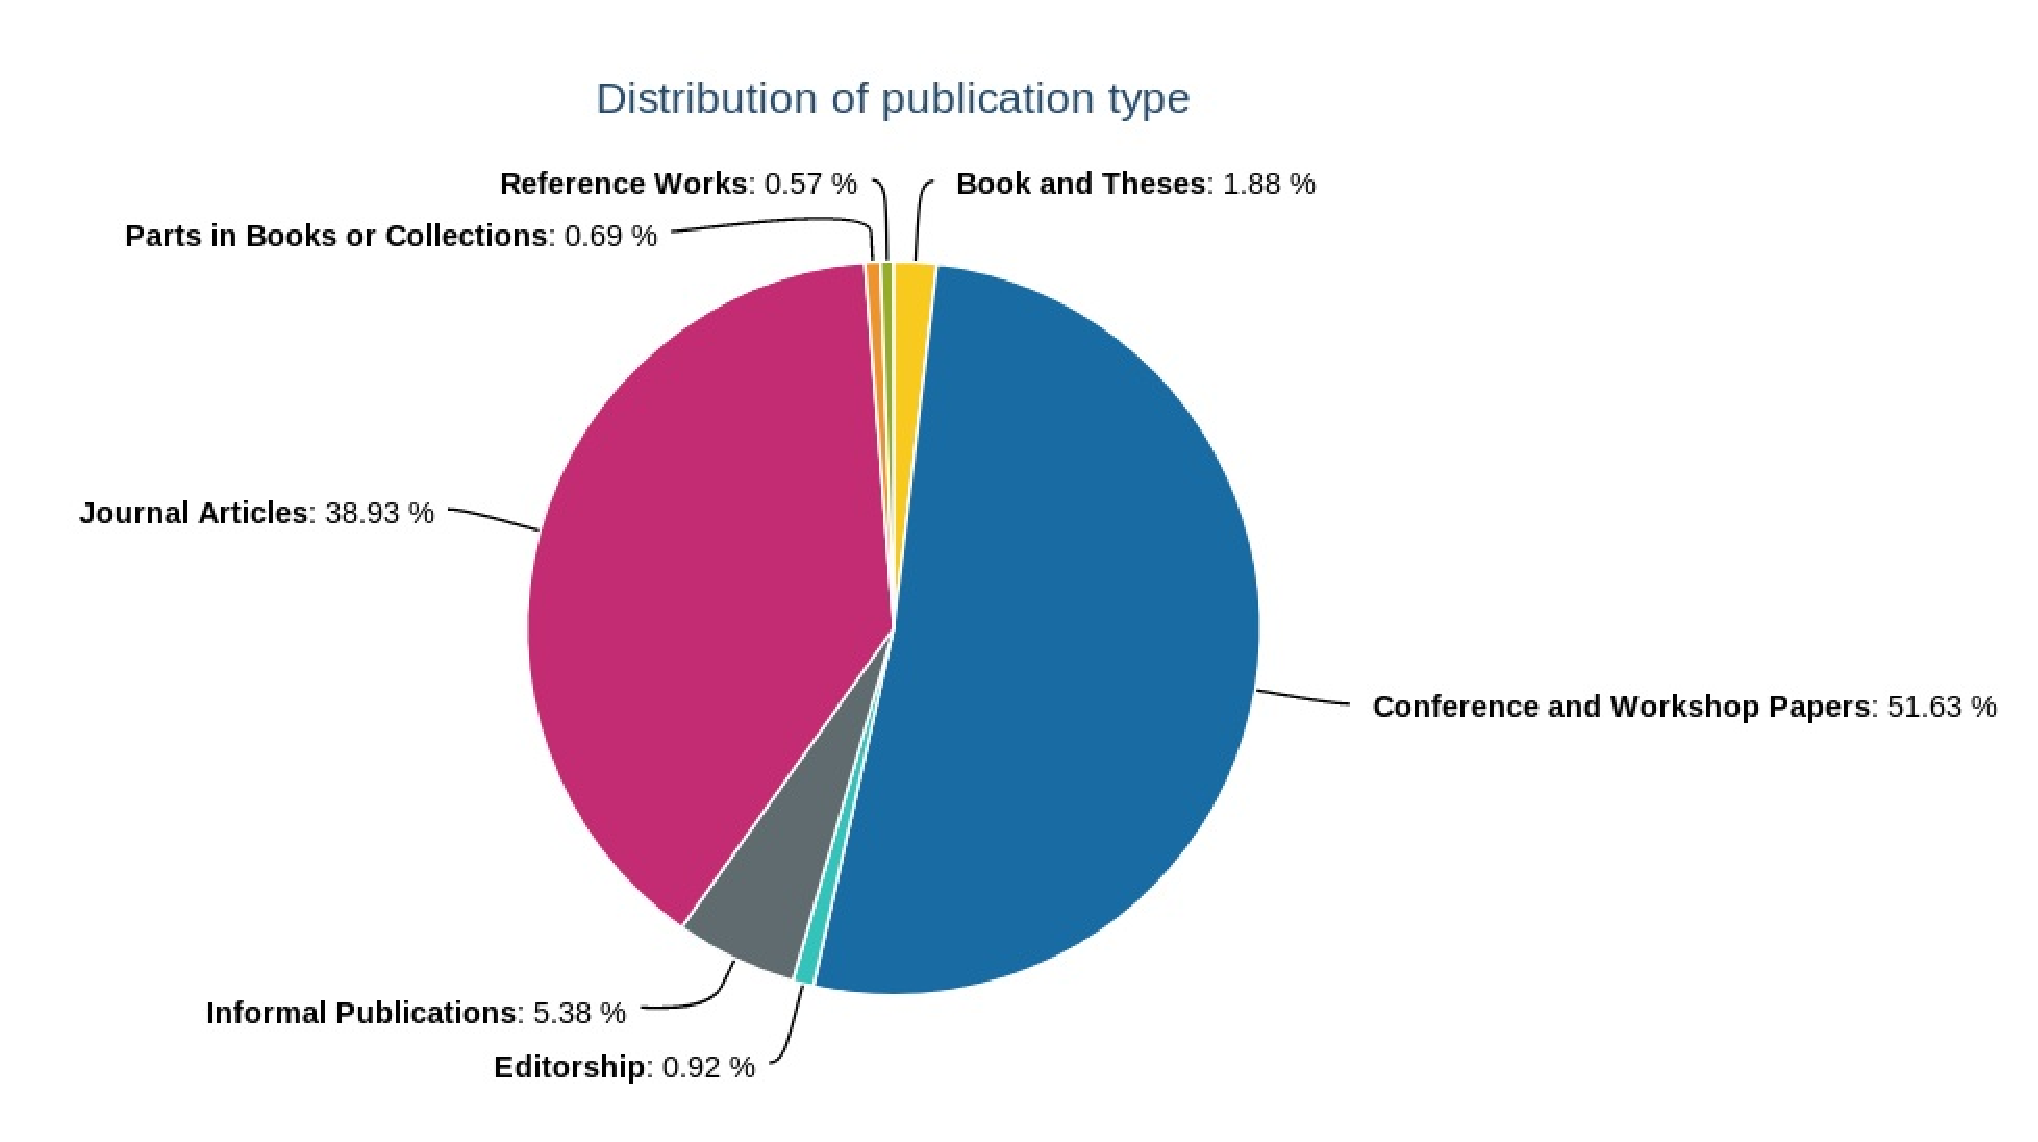
\includegraphics[width=\textwidth,height=0.6\textheight,keepaspectratio]{img/distributionofpublicationtype_2019.eps}
    \end{center}
  \end{figure}
\end{frame}

\begin{frame}{\currentname}{}\linespread{1.5}
  %note: also, the number of new entries to the dblp database per year is constantly growing; here: conference publication entries per year in the last few years always more than 150,000
  New entries to the database per year: conference and workshop papers
  \begin{figure}
    \begin{center}
      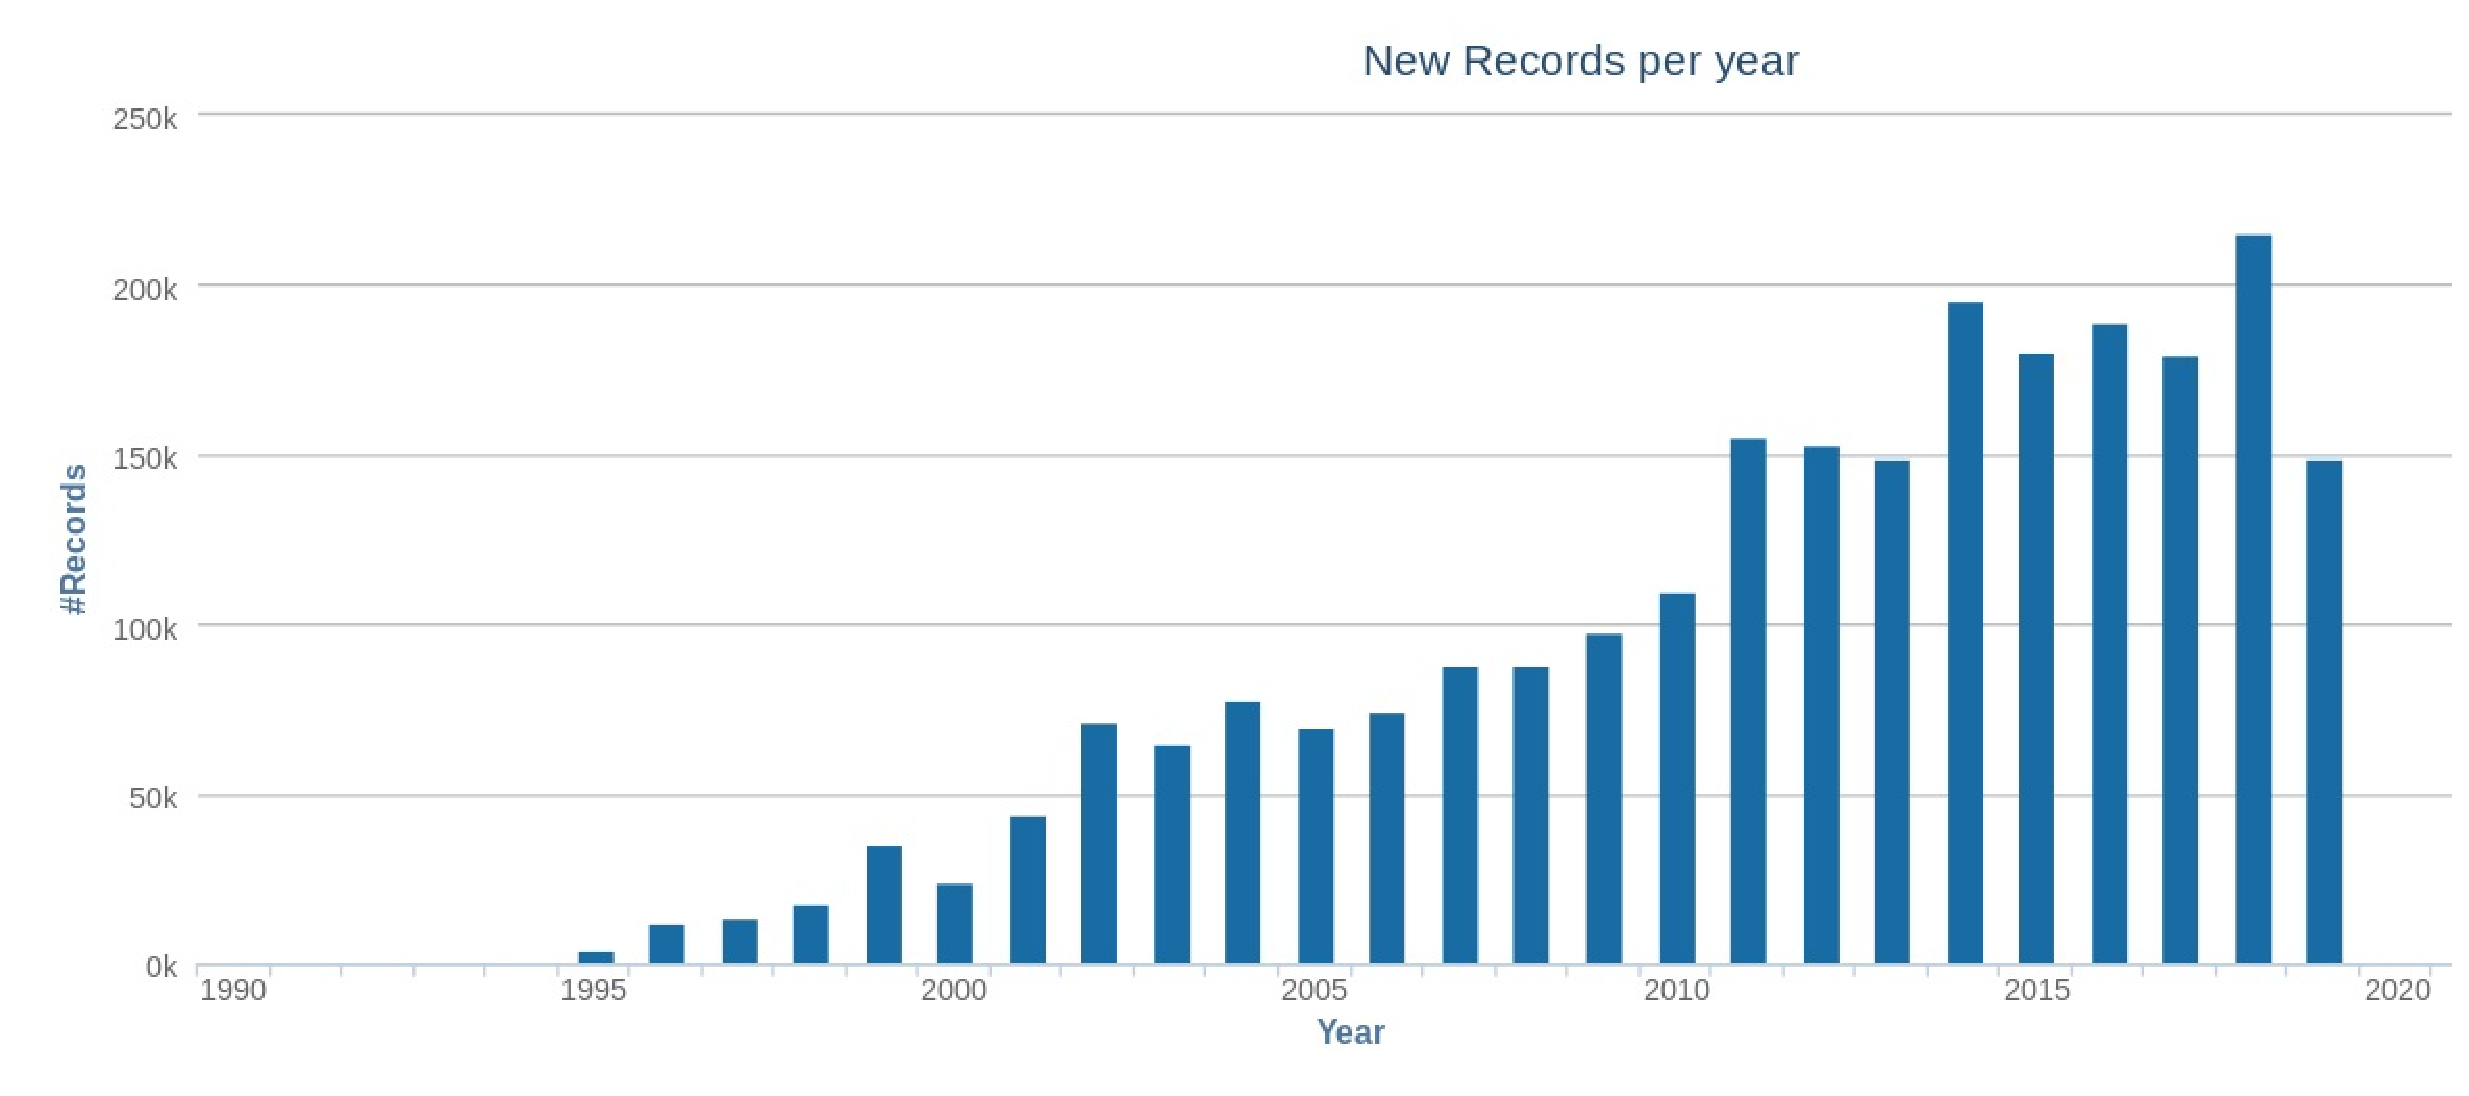
\includegraphics[width=\textwidth,height=0.8\textheight,keepaspectratio]{img/confrecordsperyear_2019.eps}
    \end{center}
  \end{figure}
\end{frame}

\begin{frame}{\currentname}{}\linespread{1.5}
  %note: these numbers show that there is a massive workload, and that dblp needs efficient monitoring at all stages of their workflow to keep up the high quality of their service
  %the sources of dblp are in particular: ...
  \begin{figure}
    \begin{center}
      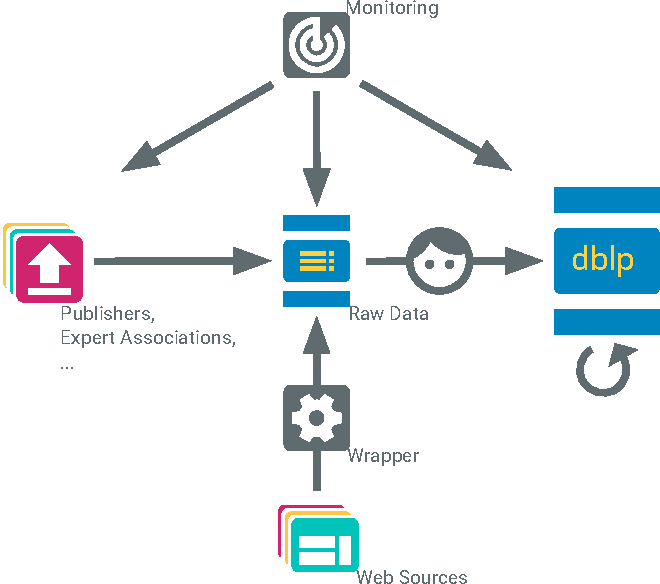
\includegraphics[width=\textwidth,height=0.8\textheight,keepaspectratio]{img/dblp-sources.pdf}
    \end{center}
  \end{figure}
\end{frame}

% \begin{frame}{\currentname}{}
%   \begin{figure}
%     \begin{center}
%       \includegraphics[width=\textwidth,height=0.8\textheight,keepaspectratio]{img/dblp_stats.eps}
%     \end{center}
%   \end{figure}
% \end{frame}
\subsection{Motivation}

\begin{frame}{\currentname}{}\linespread{1.5}
  %note: main challenges
  \begin{itemize}
    \item limited resources
    \item conferences: arbitrary intervals
    \item not all records equally important to dblp \\
      \( \rightarrow \) identify and prioritize missing data in the acquisition process

  \end{itemize}
\end{frame}

%------------------------------------------------------------------------------
\section{Research Question}
%------------------------------------------------------------------------------

\begin{frame}{\currentname}{}\linespread{1.5}
  \bigskip

  How can we find a prioritization mechanism for conference series with regard to their expected urgency for the data acquisition process at a given point in time?

  \bigskip

  \( \rightarrow \)  Ranking problem:  rank the set of conferences in descending order according to their relevance to the database
\end{frame}

%------------------------------------------------------------------------------
\section{Method}
%------------------------------------------------------------------------------
\begin{frame}{\currentname}\linespread{1.5}
  \begin{itemize}
    \item base ranking primarily dependent on temporal patterns
    \begin{itemize}
      \item relation between past event dates and dates of entry to dblp %approximate publication date
    \end{itemize}
    \item add additional factors to study influence on ranking
    \begin{itemize}
      \item loosely based on information quality / dblp quality criteria % e.g. from the quality criteria: ``The set of authors should be international.''
    \end{itemize}
  \end{itemize}

\end{frame}

\begin{frame}{\currentname}\linespread{1.5}
  Temporal patterns
  \begin{itemize}
    \item basic date-based calculation of expectancy\\
    \( \rightarrow \) delay as base scoring factor
    \item publication date of proceedings not available -- use entry date to dblp database as approximation
  \end{itemize}

  % \begin{figure}
  %   \begin{center}
  %     
\includegraphics[width=2cm,keepaspectratio]{img/november.eps}
  %   \end{center}
  % \end{figure}
\end{frame}

% %%test slide for tikz
% \begin{frame}
%
%   \begin{tikzpicture}[scale=3]
%
%     \draw[step=.5cm,gray,very thin] (-1.4,-1.4) grid (1.4,1.4);
%
%     \filldraw [gray]  (0,0) circle (2pt)
%                       (1,1) circle (2pt)
%                       (2,1) circle (2pt)
%                       (2,0) circle (2pt);
%     \draw (0,0) .. controls (1,1) .. (2,0);
%
%     \draw (-1.5,0) -- (1.5,0);
%     \draw (0,-1.5) -- (0,1.5);
%
%     \draw[loosely dotted] (0,0) circle (1cm);
%     \draw (0,0) rectangle (0.5,0.5);
%     \draw (-0.5,-0.5) rectangle (-1,-1);
%
%     \node at ( 0,2) [circle,draw] {a};
%     \node at ( 0,1) [circle,draw] {e};
%     \node at ( 0,0) [circle,draw] {i};
%     \node at ( 1,1) [rectangle,draw] {o};
%     \node at (-1,1) [rectangle,draw] {u};
%
%   \end{tikzpicture}
% \end{frame}
% %%end test slide for tikz

% \makeatletter
% %
%     % This way you can define your own conditions, for example, you
%     % could make something as `full moon', `even week', `odd week',
%     % et cetera. In principle. The math in TeX could be hard.
%     \pgfkeys{/pgf/calendar/start of year/.code={%
%         \ifnum\pgfcalendarifdateday=1\relax%
%             \ifnum\pgfcalendarifdatemonth=1\relax\pgfcalendarmatchestrue\fi%
%         \fi%
%     }}%
% %
%     % Define our own style
%     \tikzstyle{week list sunday}=[
%         % Note that we cannot extend from week list,
%         % the execute before day scope is cumulative
%         execute before day scope={%
%                \ifdate{day of month=1}{\ifdate{equals=\pgfcalendarbeginiso}{}{
%                % On first of month, except when first date in calendar.
%                    \pgfmathsetlength{\pgf@y}{\tikz@lib@cal@month@yshift}%
%                    \pgftransformyshift{-\pgf@y}
%                }}{}%
%         },
%         execute at begin day scope={%
%             % Because for TikZ Monday is 0 and Sunday is 6,
%             % we can't directly use \pgfcalendercurrentweekday,
%             % but instead we define \c@pgf@counta (basically) as:
%             % (\pgfcalendercurrentweekday + 1) % 7
%             \pgfmathsetlength\pgf@x{\tikz@lib@cal@xshift}%
%             \ifnum\pgfcalendarcurrentweekday=6
%                 \c@pgf@counta=0
%             \else
%                 \c@pgf@counta=\pgfcalendarcurrentweekday
%                 \advance\c@pgf@counta by 1
%             \fi
%             \pgf@x=\c@pgf@counta\pgf@x
%             % Shift to the right position for the day.
%             \pgftransformxshift{\pgf@x}
%         },
%         execute after day scope={
%             % Week is done, shift to the next line.
%             \ifdate{Saturday}{
%                 \pgfmathsetlength{\pgf@y}{\tikz@lib@cal@yshift}%
%                 \pgftransformyshift{-\pgf@y}
%             }{}%
%         },
%         % This should be defined, glancing from the source code.
%         tikz@lib@cal@width=7
%     ]
% %
%     % New style for drawing the year, it is always drawn
%     % for January
%     \tikzstyle{year label left}=[
%         execute before day scope={
%             \ifdate{start of year}{
%                 \drawyear
%             }{}
%         },
%         % Right align
%         every year/.append style={
%             anchor=east,
%         }
%     ]
% %
%     % Style to force giving a month a year label.
%     \tikzset{draw year/.style={
%         execute before day scope={
%             \ifdate{day of month=1}{\drawyear}{}
%         }
%     }}
% %
%     % This actually draws the year.
%     \newcommand{\drawyear}{
%         \pgfmathsetlength{\pgf@x}{\tikz@lib@cal@xshift}%
%         \pgftransformxshift{-\pgf@x}
%         % \tikzyearcode is defined by default
%         \tikzyearcode
%         \pgfmathsetlength{\pgf@x}{\tikz@lib@cal@xshift}%
%         \pgftransformxshift{\pgf@x}
%     }
% %
%     \makeatother

\begin{frame}
  \only<1>{2011}
  \only<2>{2012}
  \only<3>{2013}
  \only<4>{2014}
  \only<5>{2015}
\begin{center}
    % \begin{tikzpicture}[scale=0.6, every calendar/.style={
    %     month label above centered,
    %       month text={\textit{\%mt}},
    %       year label left,
    %   }]
    \begin{tikzpicture}[scale=0.6]

      \scriptsize
      \foreach \i in {1,...,12}
      {
        \pgfmathtruncatemacro{\y}{(\i - 1) / 4};
        \pgfmathtruncatemacro{\x}{\i - 4 * \y};
        \only<1>\calendar (cal) [dates=2011-\i-01 to 2011-\i-last, month label above centered, week list, day xshift=1.9em] at (4*\x,-4*\y);
        \only<2>\calendar (cal) [dates=2012-\i-01 to 2012-\i-last, month label above centered, week list] at (4*\x,-4*\y);
        \only<3>\calendar (cal) [dates=2013-\i-01 to 2013-\i-last, month label above centered, week list] at (4*\x,-4*\y);
        \only<4>\calendar (cal) [dates=2014-\i-01 to 2014-\i-last, month label above centered, week list] at (4*\x,-4*\y);
        \only<5>\calendar (cal) [dates=2015-\i-01 to 2015-\i-last, month label above centered, week list] at (4*\x,-4*\y);
      }

      \only<1>{\draw[red,ultra thick]($(cal-2011-06-17.south east) + (-1.2mm,1.2mm)$) rectangle ($(cal-2011-06-17.north west) + (1.2mm,-1.2mm)$){};}
      \only<1>{\draw[blue,ultra thick]($(cal-2011-09-25.south east) + (-1.2mm,1.2mm)$) rectangle ($(cal-2011-09-25.north west) + (1.2mm,-1.2mm)$){};}

      \only<2>{\draw[red,ultra thick]($(cal-2012-06-14.south east) + (-1.2mm,1.2mm)$) rectangle ($(cal-2012-06-14.north west) + (1.2mm,-1.2mm)$){};}
      \only<2>{\draw[blue,ultra thick]($(cal-2012-09-12.south east) + (-1.2mm,1.2mm)$) rectangle ($(cal-2012-09-12.north west) + (1.2mm,-1.2mm)$){};}

      \only<3>{\draw[red,ultra thick]($(cal-2013-07-26.south east) + (-1.2mm,1.2mm)$) rectangle ($(cal-2013-07-26.north west) + (1.2mm,-1.2mm)$){};}
      \only<3>{\draw[blue,ultra thick]($(cal-2013-08-22.south east) + (-1.2mm,1.2mm)$) rectangle ($(cal-2013-08-22.north west) + (1.2mm,-1.2mm)$){};}

      \only<4>{\draw[red,ultra thick]($(cal-2014-06-12.south east) + (-1.2mm,1.2mm)$) rectangle ($(cal-2014-06-12.north west) + (1.2mm,-1.2mm)$){};}
      \only<4>{\draw[blue,ultra thick]($(cal-2014-10-11.south east) + (-1.2mm,1.2mm)$) rectangle ($(cal-2014-10-11.north west) + (1.2mm,-1.2mm)$){};}

      \only<5>{\draw[red,ultra thick]($(cal-2015-06-25.south east) + (-1.2mm,1.2mm)$) rectangle ($(cal-2015-06-25.north west) + (1.2mm,-1.2mm)$){};}
      \only<5>{\draw[blue,ultra thick]($(cal-2015-09-15.south east) + (-1.2mm,1.2mm)$) rectangle ($(cal-2015-09-15.north west) + (1.2mm,-1.2mm)$){};}

      %Legende?
      % \draw[blue,ultra thick] (0,0) rectangle +(1.2mm,-1.2mm) [label=event date] {};
      % \draw[red,ultra thick] (0,0) rectangle +(1.2mm,-1.2mm) [label=entry date]{};

    %shapes examples:
    % \node [draw,regular polygon,regular polygon sides=3] {};
    % \node [draw,cloud] {};
    % \node [fill=yellow,draw,star] {};
    \end{tikzpicture}
\end{center}

\end{frame}

\begin{frame}{\currentname}\linespread{1.5}
\begin{itemize}
  \item Example conference:
  \begin{itemize}
    \item interval: 1
    \item usual month: June
    % \item last entry: 2015-06
    \item usual delay: 3 months
  \end{itemize}
  \( \rightarrow \) expected: September 2016
  \item 177 other conferences also due in September
  \item base scoring: raw delay between expected and current date; \\
  mapping of raw delay to intervals to smooth out high delays
\end{itemize}

\end{frame}

\begin{frame}{\currentname}\linespread{1.5}
  \setbeamercovered{transparent}
  \only<1>{Additional factors to refine priority ranking:}
  \only<2->{Data sets:}
  \begin{itemize}
    \item conference rating\only<3->{: CORE; Martins et al. \footfullcite{Martins:2009:AssessQualityOfConferences}}
    \item citation counts\only<4->{: Microsoft Academic Graph (MAG)}
    \item discontinuity indicator\only<5->{: self-defined, in terms of \#years since last appearance in dblp}
    \item internationality\only<6->{: self-defined, in terms of \#countries of conference venues}
    \item author prominence\only<7->{: dblp data}
  \end{itemize}
\end{frame}

% \begin{frame}{\currentname}\linespread{1.5}
%   Data sets
%   \begin{itemize}
%     \item conference rank: CORE, ???
%     \item citation counts: MAG
%     \item discontinuity indicator: self-defined, in terms of \#years since last appearance in dblp
%     \item internationality: self-defined, in terms of \#countries of conference venues
%     \item author prominence: dblp data
%   \end{itemize}
% \end{frame}

\begin{frame}{\currentname}\linespread{1.5}
  Gold standard:

  \begin{itemize}
    \item human judgments hardly practicable
    \item pseudo-relevance:
    \begin{itemize}
      \item distance in months between current month and month of ingestion into dblp
      \item mapped onto intervals
      \item inverted to give higher values to more recent entries
    \end{itemize}
  \end{itemize}
\end{frame}

\section{Our Results/Contribution}

\subsection{Main Results}

% \begin{frame}{\currentname}\linespread{1.5}
%   \begin{itemize}
%     \item every factor outperforms baseline
%     \item some fluctuation over the year
%   \end{itemize}
% \end{frame}

\begin{frame}{\currentname}\linespread{1.5}
  \begin{itemize}
    \item every factor outperforms baseline
    % \item some fluctuation over the year
  \end{itemize}
  \begin{table}[t]
  \caption{Overview on \ndcg-100 values for each month and the year's average. }\label{table/resultsMonths}
    \begin{center}
  	\csvautobooktabular[separator=semicolon]{tables/ndcg2.csv}
    \end{center}
  \end{table}
\end{frame}

\begin{frame}{\currentname}\linespread{1.5}
  \begin{table}[t]
  \caption{Comparison of \ndcg values on different cut-offs. Statistical differences to the baseline tested with two-sided t-test ($*** = p<0.001$, $** = p<0.01$, $ * = p<0.05 $).}\label{table/resultsCutoffs}
    \begin{center}
      \csvautobooktabular[separator=semicolon]{tables/ndcgcutoffs.csv}
    \end{center}
  \end{table}
\end{frame}

\subsection{Interpretation}

\begin{frame}{\currentname}\linespread{1.5}
  Best performing factors in terms of information quality:
  \begin{itemize}
    \item credibility:
    \begin{itemize}
      \item expressed through ratings
    \end{itemize}
    \item currency:
    \begin{itemize}
      \item expressed through penalty by discontinuity
    \end{itemize}
    \item popularity:
      \begin{itemize}
        \item expressed through citation, internationality and prominence scores
      \end{itemize}
  \end{itemize}
\end{frame}
%
% \subsection{Basic Ideas for Proofs/Implementation}
%
% \begin{frame}{\currentname}\linespread{1.5}
% \end{frame}
%
% \begin{frame}{\currentname}\linespread{1.5}
% \end{frame}

\section*{Summary}

\begin{frame}{\currentname}\linespread{1.5}

  % Keep the summary *very short*.
  \begin{itemize}
    \item
      We can use information quality-related features to rank conferences for data ingestion routines.
      % The \alert{first main message} of your talk in one or two lines.
    \item
    All proposed features outperform the baseline derived from ingestion delays.
      % The \alert{second main message} of your talk in one or two lines.
    % \item
    %   Perhaps a \alert{third message}, but not more than that.
  \end{itemize}

  % The following outlook is optional.
  \vskip0pt plus.5fill
  \begin{itemize}
  \item
    Outlook
    \begin{itemize}
    \item separate workshops
    \item extend approach to journals etc.
    \item Learning to Rank
    \end{itemize}
  \end{itemize}
\end{frame}

%------------------------------------------------------------------------------

\begin{frame}{Discussion}
Thank you for your attention!\\
Feel free to ask any questions now!\bigskip

Contact us:\\
\url{mandy.neumann@th-koeln.de}\\
\url{michelsc@uni-trier.de}\\
\url{philipp.schaer@th-koeln.de}\\
\url{schenkel@uni-trier.de}\bigskip

Visit \url{http://dblp.uni-trier.de}

\end{frame}

%------------------------------------------------------------------------------

\setbeamertemplate{section in toc shaded}[default][100]
  \begin{frame}{Table of contents}
  	\tableofcontents[
      currentsection,
      currentsubsection,
      subsectionstyle=hide
    ]
  \end{frame}

%------------------------------------------------------------------------------

% All of the following is optional and typically not needed.
\appendix
\section<presentation>*{\appendixname}
\subsection<presentation>*{For Further Reading}

% \begin{frame}[allowframebreaks]
%   \frametitle<presentation>{References}
%   \bibliographystyle{amsalpha}
%   \bibliography{main.bib}
% \end{frame}

% \begin{frame}[allowframebreaks]
%   \frametitle<presentation>{For Further Reading}
%
%   \begin{thebibliography}{10}
%
%   \beamertemplatebookbibitems
%   % Start with overview books.
%
%   \bibitem{Author1990}
%     A.~Author.
%     \newblock {\em Handbook of Everything}.
%     \newblock Some Press, 1990.
%
%
%   \beamertemplatearticlebibitems
%   % Followed by interesting articles. Keep the list short.
%
%   \bibitem{Someone2000}
%     S.~Someone.
%     \newblock On this and that.
%     \newblock {\em Journal of This and That}, 2(1):50--100,
%     2000.

%   \end{thebibliography}
% \end{frame}

\end{document}
